%************************************************
\chapter{Passive and Active Communications}\label{ch:passive_com}
%************************************************

In a previous chapter we learned how to exchange data with the server, since \ac{XML} and \ac{JSON} can be used for receiving as well as transmitting information.

There are two ways in which a cloud service can communicate with an application, the application can actively query the server for new information every couple of minutes or the server can passively send information to the application, without the need for interaction.

This premise builds upon the ideas discussed in \autoref{ch:conn_cloud}, since it makes use of asynchronous, bidirectional communications as well as normal HTTP requests.

\section{Active Communications}
Active Communications are very straight-forward. When the user interacts with the application and it needs to collect more data, the application makes an active request to the server asking it for this information. Examples for this behavior are searches or when the user wants to update a view with the latest information from the server. In an application like Twitter, this can be when the user refreshes the activity feed or when he searches for something.

The application can also actively send data and, if the server allows it, manipulate the data on the server. Keeping with the Twitter example, a user can create a new tweet, follow users, manipulate existing tweets and interact with other users. All of these are examples of active communications in action.

\section{Passive Communications}
On the other hand, Passive Communications require no interaction on the user part whatsoever. The server handles all the communication and administers how, when and to whom the notifications are sent.

In mobile environments, Passive Communications are often referred to as \textit{Push Notifications}, because they are "pushed" to the device rather than actively "pulled".

There are many ways of generating push notifications:
\begin{itemize}
\item You can implement your own receiver inside the application using Websockets and have a server send the notifications over this channel.
\item You can use any of the many third party libraries that handle the implementation and offer some kind of web service to handle notifications.
\item Use Google's and Apple's own services that let you easily send notifications to your users.
\end{itemize}

Each of these methods has its pros and cons, but if you want a great amount of flexibility, without the hassle of creating everything yourself, you should use Google's and Apple's own implementation. The only downside of this approach is that we can't share this code and have to implement everything twice.


\section{Our Use Case}

The use of active communications within our application is pretty obvious. The application connects to the server periodically to get new job vacancies and new companies, if there are any, and when the user searches for something specific.

The special use case comes with the push notifications. We want the user to receive a notification when a new vacancy matching previous searches is posted.

A great advantage of using each platform's own implementation for push notifications is that most of the heavy lifting is done for you and you only need to focus on the actual task at hand, meaning sending the right notification with the right content to the right person. It is also lucky for us, that despite being two completely different systems, the underlying architecture is remarkably similar.

Both systems require a unique device ID in order to match and send notifications to the user. For this, the device first registers itself with the corresponding service and receives a unique identifier. This identifier then needs to be saved on our cloud application along with the preferences for notification.

After this process is completed, our cloud service is ready to send notifications. The procedure for doing this is again very similar for both systems. The server prepares a message containing the notification contents and the device ID and sends it to Apple's or Google's Master Systems for processing.\newline
\vfill

What happens after that varies depending on the platform:

For Apple devices the notification is alive for a short period of time. This means that if the user is offline for an extended period, he will no longer receive the notification once he connects again. There is also no message queue, meaning that if a newer message arrives before the user has fetched the previous one, he will only receive the latest message.

Devices running Android don't face most of these issues. \ac{GCM} Service allows for the of definition a \ac{TTL}, which tells GCM how long to keep the message in storage before it's deleted. This value defaults to 4 weeks. And GCM does implement a queue, allowing for all sent messages to be delivered, if their \ac{TTL} hasn't expired.

\section{Implementation} 

In order to send the notifications, we need to add the specific implementation of each service to the application. 
\begin{figure}[bth]
        \myfloatalign
        \subfloat[Google Cloud Messanging]
        {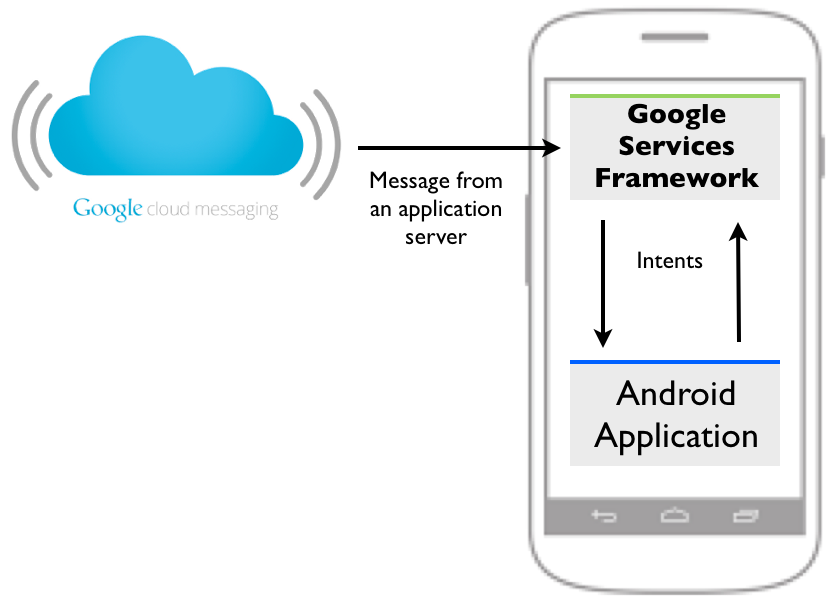
\includegraphics[width=.65\linewidth]{gfx/gcm}} \quad
        \subfloat[Apple Push Notification Service]
        {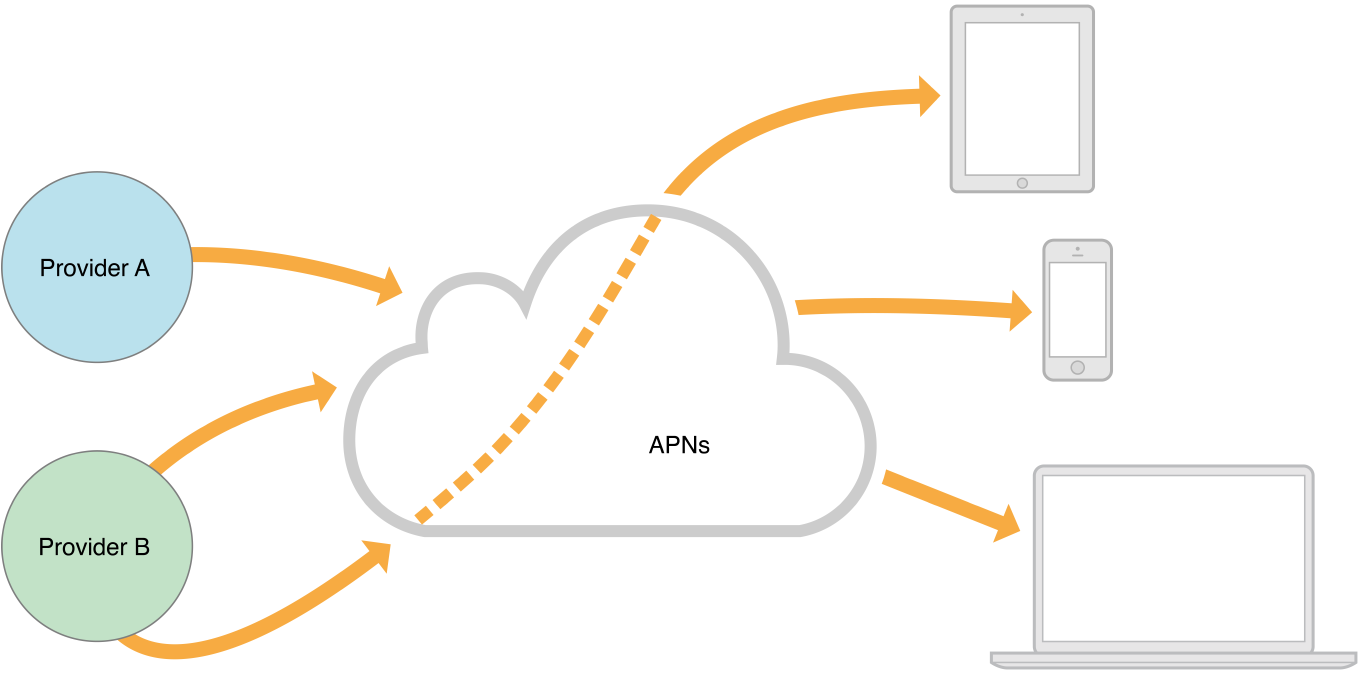
\includegraphics[width=.65\linewidth]{gfx/apns}} \\
        \caption[Cloud Messaging Services]{Cloud Messaging Services\footnotemark}\label{fig:push}
\end{figure}
\footnotetext{Source: \url{http://docs.xamarin.com/guides/cross-platform/application_fundamentals/notifications/android} \& \url{https://developer.apple.com/library/ios/documentation/NetworkingInternet/Conceptual/RemoteNotificationsPG/}}

Both services require you to register your application with them, so that you can send notifications and also require special configuration in the app's permission, so that it can receive the remote messages. Let's take a look at how the rest of the implementation is done, after the registration and permission set up.


\subsection{Android}

First thing you have to do is register the device with \ac{GCM} and save the registration ID, if it wasn't saved previously. This ID is needed in order to identify the device with our cloud service.

The \texttt{MainActivity} checks at runtime if there is no Registration ID and if the App Version has changed. In both cases the \texttt{RegisterInBackground} method gets called, in order to fetch the ID from Google.

\begin{lstlisting}[frame=lt,caption=GCM Registration, label={list:reg_and}]
void RegisterInBackground () {
	Task.Factory.StartNew (() => {
		try {
			GCM = GoogleCloudMessaging.GetInstance (ApplicationContext);
			RegID = GCM.Register (SenderID);
			storage.Put (PropertyRegID, RegID);
			SendRegistrationIdToBackend (RegID);
		} catch (Java.IO.IOException) {
			storage.Put ("failed_registration", true);
		}	
	});
}
\end{lstlisting}

Once we have the new Registration ID, we save it to the local storage and send it to the cloud service for processing. If it fails to retrieve the ID, the failure is stored, in order to avoid a registration loop.

With the unique ID saved and sent to our cloud service, we are almost ready to receive notifications from \ac{GCM}. We still need to declare the receiver for these messages and a service to actually create the notifications inside the device.\vfill

\begin{lstlisting}[frame=lt,caption=GCMBroadcastReceiver.cs, label={list:reg_and_broad}]
[BroadcastReceiver(Permission= "com.google.android.c2dm.permission.SEND")]
[IntentFilter(new string[] { "com.google.android.c2dm.intent.RECEIVE" }, Categories = new string[] {"@PACKAGE_NAME@" })]
class GCMBroadcastReceiver : WakefulBroadcastReceiver {
	public override void OnReceive (Context context, Intent intent) {
		var comp = new ComponentName (context.PackageName, typeof(GCMIntentService).Name);
		StartWakefulService (context, intent.SetComponent (comp));
		ResultCode = Result.Ok;
	}
}
\end{lstlisting}

The receiver registers itself with the application to receive external messages only from \ac{GCM} and when it receives a message, it starts a special service that will keep the phone from sleeping by passing it an Intent to open the \texttt{GCMIntentService}.

\begin{lstlisting}[frame=lt,caption=GCMIntentService.cs, label={list:reg_and_serv}]
[Service]
class GCMIntentService : IntentService {
	public const int NotificationID = 1;
	NotificationManager NotificationManager;
	NotificationCompat.Builder Builder;
	protected override void OnHandleIntent (Intent intent) {
		var extras = intent.Extras;
		gcm = GoogleCloudMessaging.GetInstance(this);
		var messageType = gcm.GetMessageType(intent);
		if (!extras.IsEmpty) {
			if (GoogleCloudMessaging.MessageTypeMessage.Equals(messageType)) {
				SendNotification("New Job available: " + extras);
			}
		}
		GCMBroadcastReceiver.CompleteWakefulIntent(intent);
	}
	void SendNotification(String msg) {
		NotificationManager = (NotificationManager) GetSystemService(Context.NotificationService);
		var contentIntent = PendingIntent.GetActivity(this, 0,
			new Intent(this,typeof(MainActivity)),0);
		Builder = new NotificationCompat.Builder (this)
			.SetSmallIcon (Resource.Drawable.action_mhm)
			.SetContentTitle ("MHM Notification")
			.SetStyle (new NotificationCompat.BigTextStyle().BigText(msg))
			.SetContentText (msg)
			.SetLights (8, 600, 500);
		Builder.SetContentIntent(contentIntent);
		NotificationManager.Notify(NotificationID, Builder.Build());
	}
}
\end{lstlisting}

Once the service has been opened it fetches all the data from the message and prepares a notification to be shown. Inside this notification is the Intent to open the \texttt{MainActivity} of our application and show the latest Job Offer that was sent to the device. 

\subsection{iOS}  

The beginning of the procedure for iOS is almost the same. We need to register the device with Apple and save the unique token that we receive from the server. There is a very big advantage for iOS when it comes to setting up the notifications. It has a built in method that gets called form the \texttt{AppDelegate} that takes care of retrieving the token for you, you just need to save it somewhere and send it to the cloud service once the token is ready.

\begin{lstlisting}[frame=lt,caption=Modified AppDelegate, label={list:reg_ios}]
public class AppDelegate : UIApplicationDelegate {
	[...]
	public override bool FinishedLaunching (UIApplication application, NSDictionary launchOptions) {
		[...]
		UIApplication.SharedApplication.RegisterForRemoteNotificationTypes (UIRemoteNotificationType.Alert 
			| UIRemoteNotificationType.Badge 
			| UIRemoteNotificationType.Sound);

		if (launchOptions != null) {
			var dictionary = launchOptions.ObjectForKey (UIApplication.LaunchOptionsRemoteNotificationKey);
			if (dictionary != null) {
				Console.WriteLine ("Received Dictionary: " + dictionary);
				PublicationViewController.HandleNotification (dictionary);			
			}
		}		
		return true;
	}
	public override void RegisteredForRemoteNotifications (UIApplication application, NSData deviceToken) {
		TokenHandler.SetToken (deviceToken);
	}
	public override void DidReceiveRemoteNotification (UIApplication application, NSDictionary userInfo, System.Action<UIBackgroundFetchResult> completionHandler) {
		Console.WriteLine ("Received info: " + userInfo);
		PublicationViewController.HandleNotification (dictionary);
	}
}
\end{lstlisting}

Once the application tries to register with Apple, it presents the user with a choice to allow or disallow Push Notifications. If the user doesn't allow it, we will not be able to send Push Notifications to this device. This setting can be changed by the user inside the iOS Notification Center.

Inside the \texttt{AppDelegate} File is all the code needed handle the notifications. Unlike Android, there is no need to manually create and show a notification to the user. This behavior is handled by the operating system. There is however the drawback that you cannot modify the default notification. Android does allow you to modify the notification and also add secondary and tertiary action buttons to a notification.

\section{Final Thoughts}

After implementing both systems I can say that Apple makes it easier to set up Push Notifications, but doesn't give you the flexibility and configurability that Android does. 

Due to length constraints and scope of this work I cannot show you all the code and all the steps necessary in order to get Push Notifications working on both platforms, and keep in mind that we are only talking about client side implementation here. There is a lot to be said about the server side implementation that is supposed to handle everything. The server needs to implement the connection protocols to each service, save each Unique Device ID to the database, match user saved searches with each new Publication posted and trigger notifications for each matching Publication. That task alone is worthy of its own book.


 





